\subsection{Convolutional Neural Network}
    \subsubsection{Model Desciption}
        The following section will describe the TensorFlow Keras
        \cite{tensorflow2015-whitepaper} model used in the prototype of the
        Image Classification tool alongside some results.  
        After  loading  the  images,  the  dataset  was  split  into  a
        training and testing set, 80\% and 20\% respectively. The model
        receives 180x180x3 standardized RGB images with a batch size of
        32. \\
        The dataset’s small size will make it prone to overfitting.
        Data augmentation,  a technique for generating additional training
        data by randomly transforming the existing data, is used to
        overcome this issue. Figure \ref{augmentation} shows an example of an image  being
        rotated to generate additional images to the existing dataset.
        Overfitting is also avoided by using another technique called
        dropout. This technique randomly sets the activation function to
        0. This forces the model to learn redundancy for everything. \\

        \begin{figure}[H]
            \caption{Data Augmentation}
            \centering
            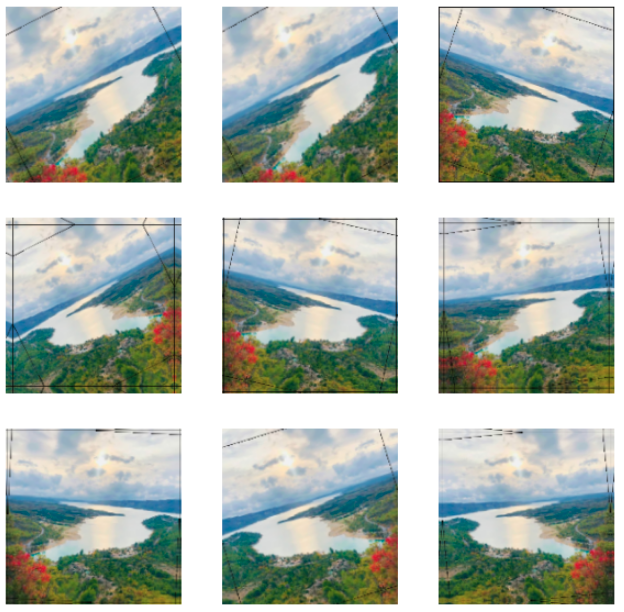
\includegraphics[scale=0.28]{Augmentation.png}
            \label{augmentation}
        \end{figure}

        The model contains three convolutional layers with a rectified linear
        unit (ReLU) activation function, each followed by a pooling layer
        to lower down the spatial dimension of the input volume for next
        layers. The layer then ends with a flattening layer and two dense
        layers to reduce the outputs to the amount of classes, in this
        case 5. The following figure shows a summary of the whole model.

        \begin{figure}[H]
            \caption{model Summary}
            \centering
            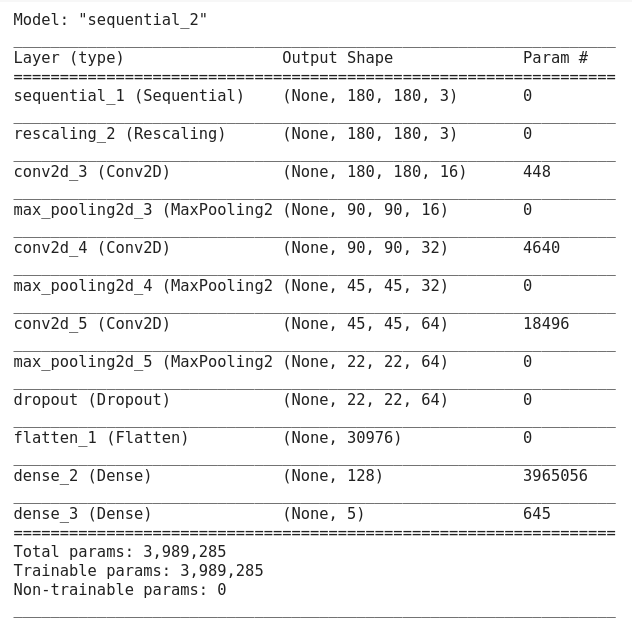
\includegraphics[scale=0.3]{Summary.png}
            \label{summary}
        \end{figure}

    \subsubsection{Results}
    The results in the next figure show how the model has reached
    nearly 80\% accuracy with very little data. More images could be
    added to make such a model more accurate.

    \begin{figure}[H]
        % \caption{model Summary}
        \centering
        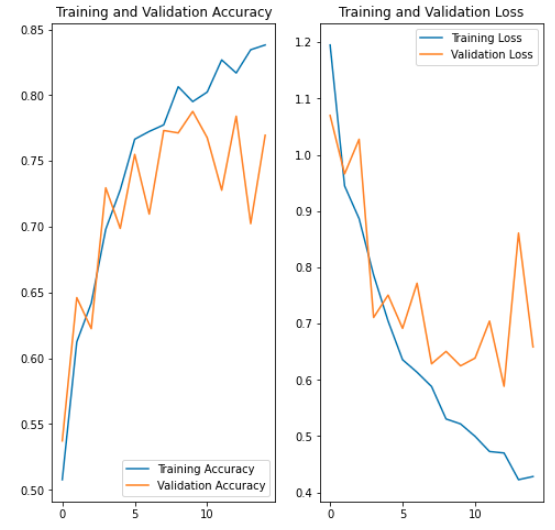
\includegraphics[scale=0.35]{Results.png}
        \label{ModelResults}
    \end{figure}

    The following shows an output of the prototype when given an image
    of a beach found on the internet:
    \url{https://selfgrowth.info/photos/free-beach-photos-without-copyright/big-beach-illustrations-free-royalty6361.jpg}

    \begin{figure}[H]
        % \caption{model Summary}
        \centering
        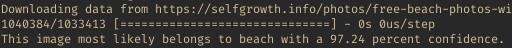
\includegraphics[scale=0.5]{sample.png}
        \label{oneOutput}
    \end{figure}

\subsection{Preference Gathering}
        This section will describe an example of the score calculation based
        on user criteria. Initially, the application asks the user certain
        preferences such as:
        \begin{enumerate}
            \item The trip budget
            \item Moderation of activities (How busy the trip needs to be)
            \item Users’ characteristics (based on Instagram Results)
            \\ A user’s score for category \textbf{A} would be
            calculated by gathering the total number of \textbf{A}
            labelled photos over the total number of photos. 
            \item Number of people
            \item Where the user is going
            \item Date and time the user will be going
        \end{enumerate}

        \begin{figure}[H]
            \caption{The following figure includes some sample user preferences        }
            \centering
            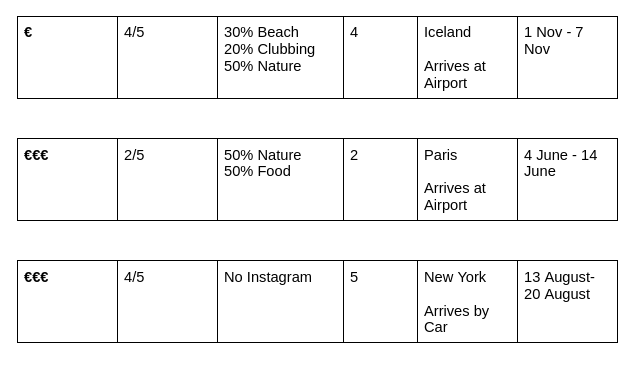
\includegraphics[scale=0.41]{SampleResults.png}
            \label{dataset}
        \end{figure}

        Each Activity will contain its own details upon which a
        score is calculated. Some example of such parameters include:
        \begin{enumerate}
            \item Cost
            \item How close is the place to the user’s characteristics (from Instagram)
            \item At what time is the place open
            \item Approximately the amount of time people spend there (even based on user’s moderation)
            \item Place Importance
            \item What type of Weather is the place accessible
            \item Time to travel from the previous location
            \item Place reviews
            
        \end{enumerate}

        \begin{figure}[H]
            \caption{The following figure includes some sample activity details}
            \centering
            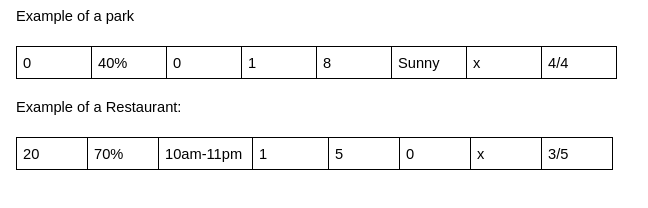
\includegraphics[scale=0.41]{SamplePlace.png}
            \label{dataset}
        \end{figure}

        % \begin{figure}[H]
        %     \caption{The following figure includes some sample activity details}
        %     \centering
        %     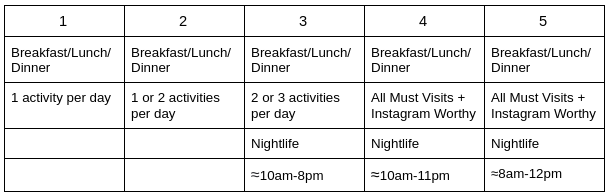
\includegraphics[scale=0.41]{UserModeration.png}
        %     \label{d}
        % \end{figure}
